\documentclass[12pt, a4paper, twoside]{article}
\usepackage{tikz}
\usepackage{amsmath}
\usepackage{amssymb}
\usepackage{gensymb}

\begin{document}
\begin{titlepage}
  \begin{center}
    \vspace*{5cm}
    \huge\textbf{Angewandte Mathematik}\\
    \vspace{0.5cm}
    Auftrag Kurven\\
    \date\\
    \vspace{2cm}
  \end{center}
\end{titlepage}
\section{Aufgabenbeschreibung}
Der Punkt M dreht sich im Abstand von 6 um den Ursprung mit Winkelgeschwindigkeit 1 im Gegenuhrzeigersinn.
Der Punkt P derht um M im Abstand von 4 mit Winkelgeschwindigkeit w um M im Uhrzeigersinn.
Die Anfangsposition von P ist (2, 0).

\begin{center}
  Startposition:
\end{center}
\begin{center}
  \begin{tikzpicture}
    \filldraw
    (0,0) circle (0.08cm) node(O)[left] {O}
    (0:3cm) circle (0.08cm) node[left] {M}
    (0:3cm) ++(180:2.5cm) circle (0.08cm) node[right] {P}
    ;


    \draw
    (0, 0) circle (3cm)
    (0:3cm) circle (2.5cm)
    ;
  \end{tikzpicture}
\end{center}



\begin{center}
  Position nach $t$ Zeit:
\end{center}
\begin{center}
  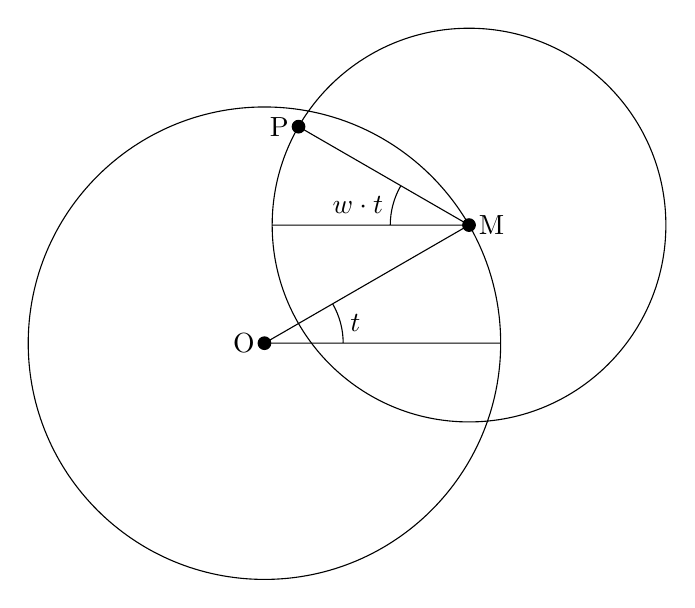
\begin{tikzpicture}
    \filldraw
    (0,0) circle (0.08cm) node(O)[left] {O}
    (30:3cm) circle (0.08cm) node[right] {M}
    (30:3cm) ++(150:2.5cm) circle (0.08cm) node[left] {P}
    ;

    \draw
    (0, 0) circle (3cm)
    (30:3cm) circle (2.5cm)
    ;

    \draw
    (30:3cm) ++(180:1cm) arc (180:150:1) node[pos=0.5, left]{$w\cdot t$}
    (30:3cm) -- ++(150:2.5cm)
    (30:3cm) -- ++(180:2.5cm)

    (1cm, 0) arc (0:30:1) node[pos=0.5, right]{$t$}
    (30:3cm) -- (0, 0) -- (3cm, 0)
    ;

  \end{tikzpicture}
\end{center}
\pagebreak
\section{Parameterdarstellung}
Für die Parameterdarstellung suche ich den Ortsvector $\vec{P}$.

\begin{align*}
  \overrightarrow{P} & = \overrightarrow{M} + \overrightarrow{MP} \\
\end{align*}

Das ist eindeutig weswegen es stimmt.
Der Vector vom Ursprung zu einem beliebigen Vector $\overrightarrow{V}$, addiert zum Vector $\overrightarrow{VP}$ wird gleich P sein.
\\

\begin{align*}
  \overrightarrow{M} & = \begin{pmatrix}
    \cos(t) \cdot 6
    \\
    \sin(t) \cdot 6
  \end{pmatrix} \\
\end{align*}

Der Punkt $M$ bewegt sich mit einer Winkelgeschwindigkeit von 1 auf einem Kreis mit einem Radius von 6.
Eine Bewegung mit der Winkelgeschwindigkeit von 1 heisst, dass sich der Punkt in einer Zeiteinheit um 1 Winkelgrad auf der Kreisbahn engtlangbewegt.
Die sinus und cosinus Funktionen geben die x, respektive die y Koordinaten an für Punkte auf dem Einheitskreis, die mit dem Ursprung und dem Punkt (0, 1) einen bestimmten Winkel $\gamma$ einschliessen.
Wir können $t$ als Zeit nehmen, und in die cosinus Funktion einsetzen für die x Koordinate auf dem einheitskreis, und in die sinus Funktion einsetzen für die y Koordinate auf dem Einheitskreis.
Da wir aber einen Kreis mit radius 6 möchten, multiplizieren wir diesen Vector mit 6.
Somit werden alle Punkte 6mal so weit vom Ursprung sein wie auf dem Einheitskreis, und unser Kreis nimmt einen Radius von 6 an.

\begin{align*}
  \overrightarrow{MP} & = \begin{pmatrix}
    -\cos(w\cdot t) \cdot 4
    \\
    \sin(w\cdot t) \cdot 4
  \end{pmatrix}
\end{align*}
\\

Der Punkt $P$ bewegt sich mit einer Winkelgeschwindigkeit von $w$ auf einem Kreis mit dem Radius von 4.
Das heisst, das hier im Gegensatz zu vorher $t$ nicht einfach als Winkel eingesetzt werden kann, sondern es noch mit $w$ multipliziert werden muss.
Ausserdem muss die x Koordinate mit -1 multipliziert werden, da sich der punkt $P$ im Uhrzeigersinn dreht.

\begin{align*}
  \overrightarrow{P} & = \overrightarrow{M} + \overrightarrow{MP}               \\
  \overrightarrow{P} & = \begin{pmatrix}
    \cos(t) \cdot 6
    \\
    \sin(t) \cdot 6
  \end{pmatrix} + \begin{pmatrix}
    -\cos(w\cdot t) \cdot 4
    \\
    \sin(w\cdot t) \cdot 4
  \end{pmatrix} \\
  \overrightarrow{P} & = \begin{pmatrix}
    \cos(t)\cdot 6 - \cos(w\cdot t)\cdot 4
    \\
    \sin(t)\cdot 6 + \sin(w\cdot t)\cdot 4
  \end{pmatrix}
\end{align*}
\\

Die Parameterdarstellung von $P$ kann einfach aus dem Ortsvector bestimmt werden.

\begin{align*}
  \begin{cases}
    \cos(t)\cdot 6 - \cos(w\cdot t)\cdot 4
    \\
    \sin(t)\cdot 6 + \sin(w\cdot t)\cdot 4
  \end{cases}
\end{align*}
\\

Es fehlt noch der Definitionsbereich.
Der Punkt $M$ ist am selben Ort, wenn $\mod{\frac{t}{2\pi}} = 0$.
Das ist so, denn $M$ braucht $2\pi$ Zeit für eine Runde.
$P$ braucht aber $2\pi \cdot w$ Zeit für eine Runde, also ist es am selben Ort relativ zu $M$ wenn $\mod{\frac{t}{2\pi \cdot w}} = 0$ stimmt.
Der Definitionsbereich geht also von null, bis zur tiefsten Zahl die beide Gleichungen erfüllt.\\
\begin{align*}
  t \in \{0, \min(x\in\mathbb{R} | \mod{\frac{x}{2\pi}} = 0 \land\mod{\frac{x}{2\pi \cdot w}} = 0)\} \\
\end{align*}
\\

Die ganze Parameterdarstellung:
\begin{align*}
  \begin{cases}
    \cos(t)\cdot 6 - \cos(w\cdot t)\cdot 4
    \\
    \sin(t)\cdot 6 + \sin(w\cdot t)\cdot 4
  \end{cases}t \in \{0, \min\{x\in\mathbb{R} | \mod{\frac{x}{2\pi}} = 0 \land\mod{\frac{x}{2\pi \cdot w}} = 0\}\} \\
\end{align*}
\\

\pagebreak
\section{Beispiele}
Mithilfe von Visualisationstools wie GeoGebra oder tikz in \LaTeX können wir Kurven dieser Parameterdarstellung mit gegebenen $w$ Werten visualisieren.
\par
$w = 3.4$:
\begin{center}
  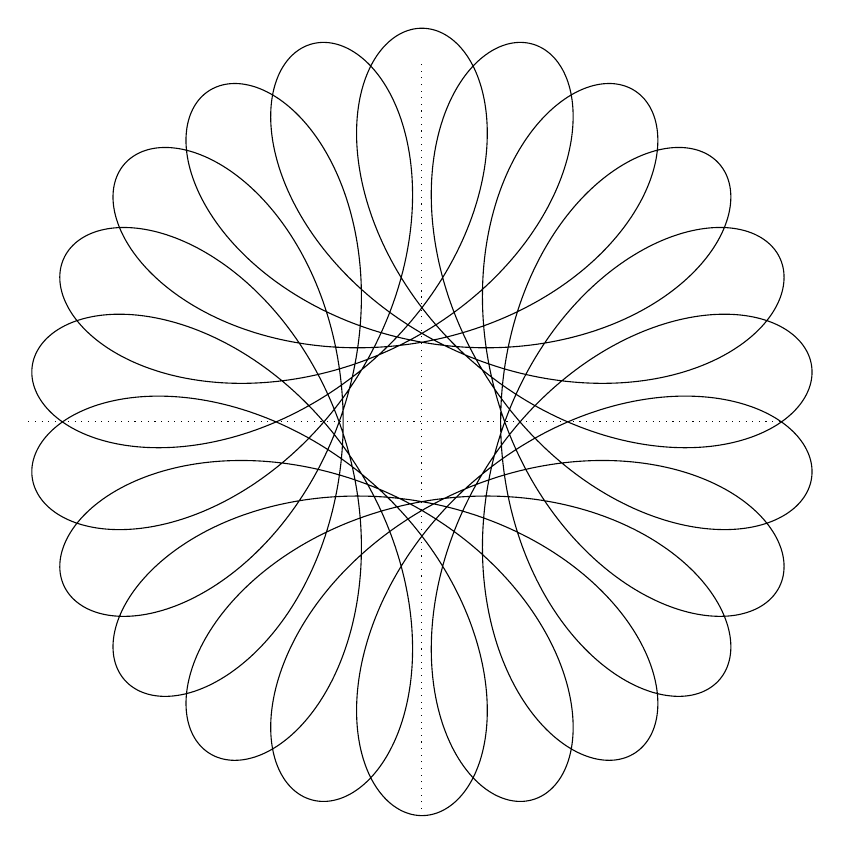
\begin{tikzpicture}
    \draw [scale=0.5,domain=0:2000,samples=4000,variable=\t]
    plot ({cos(\t)*6-cos(3.4*\t)*4}, {sin(\t)*6+sin(3.4*\t)*4})
    ;
    \draw [style=dotted]
    plot ({\x }, {0})
    plot ({0}, {\x})
    ;
  \end{tikzpicture}
\end{center}

$w = 1.5$:
\begin{center}
  \begin{tikzpicture}
    \draw [scale=0.5,domain=0:2000,samples=4000,variable=\t]
    plot ({cos(\t)*6-cos(1.5*\t)*4}, {sin(\t)*6+sin(1.5*\t)*4});

    \draw [style=dotted]
    plot ({\x }, {0})
    plot ({0}, {\x})
    ;
  \end{tikzpicture}
\end{center}
$w = 2.5$:
\begin{center}
  \begin{tikzpicture}
    \draw [scale=0.5,domain=0:2000,samples=4000,variable=\t]
    plot ({cos(\t)*6-cos(2.5*\t)*4}, {sin(\t)*6+sin(2.5*\t)*4});

    \draw [style=dotted]
    plot ({\x }, {0})
    plot ({0}, {\x})
    ;
  \end{tikzpicture}
\end{center}

\section{Anfangsgeschwindigkeit und Anfangswinkel}
Die Anfangsgeschwindigkeit ist die Länge vom Tangentialvector $\overrightarrow{r}'(t)$ bei $t=0$.
Der Anfangswinkel ist der Winkel von diesem Vector.

\begin{align*}
  \overrightarrow{r}(t)  & = \begin{pmatrix}
    x(t)
    \\
    y(t)
  \end{pmatrix} \\
  \overrightarrow{r}(t)  & = \begin{pmatrix}
    \cos(t)\cdot 6 - \cos(w\cdot t)\cdot 4
    \\
    \sin(t)\cdot 6 + \sin(w\cdot t)\cdot 4
  \end{pmatrix} \\
  \overrightarrow{r}'(t) & = \begin{pmatrix}
    x'(t)
    \\
    y'(t)
  \end{pmatrix} \\
  \overrightarrow{r}'(t) & = \begin{pmatrix}
    \sin(w\cdot t)\cdot w\cdot 4 - \sin(t)\cdot 6
    \\
    \cos(w\cdot t)\cdot w\cdot 4 + \cos(t)\cdot 6
  \end{pmatrix} \\
  \overrightarrow{r}'(0) & = \begin{pmatrix}
    0
    \\
    w\cdot 4 + 6
  \end{pmatrix} \\
\end{align*}

Die Länge von $\overrightarrow{r}'(0)$ ist $w\cdot 4 + 6$, und der Winkel senkrecht.
Somit ist die Anfangsgeschwindigkeit $w\cdot 4 + 6$, und der Anfangswinkel 90\textdegree, angenommen dass $w$ nicht negativ ist, in welchem fall der Anfangswinkel 270\textdegree wäre.
\end{document}
